\documentclass[a4paper]{article}
\usepackage{af}

\usepackage{xparse}
\usepackage{multirow}
\usepackage{longtable}
\usepackage{tikz}
\usepackage{tikz-qtree}
\usepackage{pbox}
\newlength\myheight
\newlength\mydepth
\settototalheight\myheight{Xygp}
\settodepth\mydepth{Xygp}
\setlength\fboxsep{0pt}
\newcommand*\inlinegraphics[1]{%
  \settototalheight\myheight{Xygp}%
  \settodepth\mydepth{Xygp}%
  \raisebox{-\mydepth}{\includegraphics[height=\myheight]{#1}}%
}
\usepackage[most]{tcolorbox}
\tcbset{
    frame code={}
    center title,
    left=0pt,
    right=0pt,
    top=0pt,
    bottom=0pt,
    colback=blue!26,
    colframe=white,
    width=\dimexpr\textwidth\relax,
    enlarge left by=0mm,
    boxsep=5pt,
    arc=0pt,outer arc=0pt,
}
\usetikzlibrary{arrows,shapes,positioning,shadows,trees}


%%
% Document structure, use \input for document content
%%

\newcommand{\deviceName}        {Azure Sphere}
\newcommand{\customer}          {AF Göteborg}

% af.sty parameters
\newcommand{\authorCommand}     {Jianyuan Ma}
\newcommand{\DocumentName}      {\titleCommand - \deviceName}
\newcommand{\phoneCommand}      {+46 10 505 0000}
\newcommand{\mobileCommand}     {}
\newcommand{\emailCommand}      {--@afconsult.com}
\newcommand{\projectIDCommand}  {}
\newcommand{\clientCommand}     {\customer}
\newcommand{\subtitleCommand}   {\deviceName}



% Change to correct values according to project

\newcommand{\titleCommand}      {Software Design Description}

\begin{document}
\section{Introduction}
\subsection{What is Azure Sphere}
Azure Sphere is a secured, high-level application platform with built-in communication and security features for internet-connected devices.

Azure Sphere introduces a new class of secured, connected, crossover MCU, which integrates real-time processing capabilities with a high-level 
operating system. Together with the application platform and enables product manufacturers to create secured, internet-connected device, so that
it can be updated, controlled, monitored, and maintained remotely. By embedding the MCU in a connected device, either alongside or in place of 
existing MCU(s), product manufacturers gain enhanced security, productivity, and opportunity. For example:
\begin{itemize}
    \item A secured application environment and authenticated connection can minimize the security risks from the spoofing, rogue software or denial of 
    service attacks.
    \item Software updates can be automatically deployed over the air to any connected device to provide new functionalities ,fix problems or counter 
    emerging methods of attacks, thus enhancing the productivity of support personnel.
    \item The cloud can diagnosing problems and designing new products over a secured connection, thus increasing the opportunity for product service, 
    positive customer interactions, and future development.
\end{itemize}

The Azure Sphere Security Service provides a safely and securely connect to the cloud and web. The service ensures that the device boots only with an authorized 
version of genuine, approved software. In addition, it provides a secured channel through which Microsoft can automatically download and install operating system 
updates to deployed devices in the field to mitigate security issues. Neither manufacturer nor end-user intervention is required, thus preventing a common security gap.

To read more about the Azure Sphere Security Service, please visit \href{https://docs.microsoft.com/en-us/azure-sphere/product-overview/azure-sphere-seven-properties}{Azure Sphere and the Seven Properties}


\newpage

\section{Prerequisites}
\begin{itemize}
    \item An Azure Sphere development kit
    \item A PC running Windows 10 Anniversary Update or later
    \item Visual Studio 2017 Enterprise, Professional, or Community, version 15.7 or later
\end{itemize}

Download the Azure Sphere SDK for Visual Studio Preview.
Once you’ve completed the download, follow the next chapter to install Azure Sphere and set up your board.
\newpage

\section{Install}
\label{sec:install}
\subsection{Set up you board and install SDK}

\subsubsection{Connect the board}
The development board connects to a PC through USB. The first time you plug in the board, the drivers should be automatically downloaded and installed.if the drivers are not installed automatically, right-click on the device name in Device Manager and select Update driver. Alternatively, you can download the drivers \hyperlink{https://www.ftdichip.com/Drivers/VCP.htm}{FTDI}. Choose the driver that matches your Windows installation (32- or 64-bit).

To verify installation, open Device Manager. You should be able to see three USB Serial Ports. The numbers on your COM ports may be different from those in the figure.
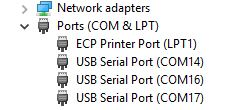
\includegraphics{COMPorts.JPG}

\subsubsection{Install the Azure Sphere SDK Preview for Visual Studio}
Azure\_Sphere\_SDK\_Preview\_for\_Visual\_Studio.exe installs the complete Azure Sphere software development kit (SDK).

To install the SDK:
\begin{enumerate}
    \item \hyperlink{https://aka.ms/AzureSphereSDKDownload}{Download the Azure Sphere SDK Preview for Visual Studio} from Visual Studio Marketplace if you have not already done so. Save the downloaded file on your PC.
    \item Run Azure\_Sphere\_SDK\_Preview\_for\_Visual\_Studio.exe from the download to install the SDK. Agree to the license terms and select Next.
    \begin{figure}[h]
    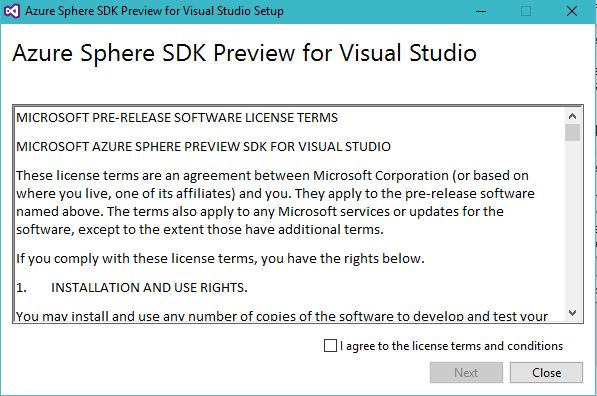
\includegraphics[scale=0.7]{SDK1.JPG}
    \end{figure}
    \newpage
    \item Click Install to begin installation.
    \begin{figure}[h]
    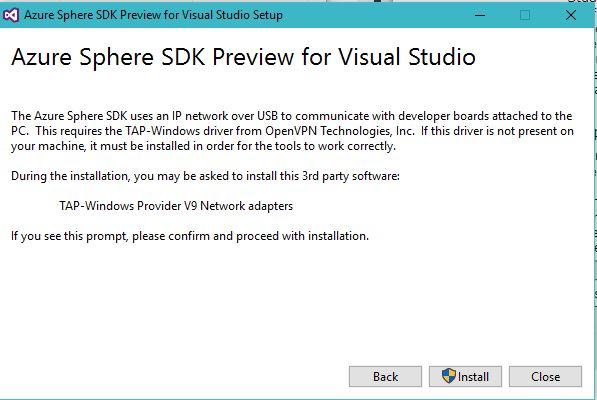
\includegraphics[scale=0.7]{SDK2.JPG}
    \end{figure}
    \newline
    If the message "This product requires Visual Studio 2017, Version 15.7 or newer" appears, ensure that Visual Studio 2017 version 15.7 or more recent is installed on your PC.

    The message "No product to install SDK on" may appear if you do not have Visual Studio version 15.7 or newer installed, or if you have just installed Visual Studio for the first time. If you see this message, either update your Visual Studio installation if necessary or restart your PC and return to this step.
    \item Accept the elevation prompt if one appears.
    \item When setup completes, restart your PC if the setup application requests it. The SDK is installed to all compatible editions of Visual Studio on your PC. The SDK requires Visual Studio version 15.7 or later.
    
\end{enumerate}

\subsection{Update OS}
If the Azure Sphere device has never been used, it most likely needs to update the OS. Follow the steps to update the Azure Sphere OS.
\begin{enumerate}
    \item Connect the board to the PC by USB.
    \item Open an Azure Sphere Developer Command Prompt. It appears in the Start menu under Azure Sphere.
    \item Issue the following command to update the Azure Sphere OS:
        \begin{lstlisting}[language=bash]
            azsphere device recover
        \end{lstlisting}
    You should see output similar to this:
        \begin{lstlisting}[language=bash]
            Starting device recovery. Please note that this may take up to 10 minutes.
            Board found. Sending recovery bootloader.
            Erasing flash.
            Sending images.
            Sending image 1 of 16.
            Sending image 2 of 16.
            . . . 
            Sending image 16 of 16.
            Finished writing images; rebooting board.
            Device ID: <GUID>
            Device recovered successfully.
            Command completed successfully in 00:02:37.3011134.
        \end{lstlisting}
\end{enumerate}

\subsubsection{Set up an account for Azure Sphere}
Azure Sphere uses Azure Active Directory (AAD) to enforce enterprise access control. Therefore, to use Azure Sphere, you need a Microsoft work or school account (sometimes called an organizational account) that is associated with an AAD.

The ÅF account is Microsoft work account, to find out you can use the account, open an Azure Sphere Developer Command prompt (on the Start menu under Azure Sphere) and sign in to Azure Sphere with your work or school account:
\begin{lstlisting}[language=bash]
    azsphere login
\end{lstlisting}
In response, azsphere prompts you to pick an account. Choose the ÅF account and type your password if required. If you see a dialog box requesting that an admin grant permission to use the Azure Sphere Utility, you'll need to log in as an administrator or obtain admin approval.

If login succeeds, the command returns a list of the Azure Sphere tenants that are available for you. You should see the similar output to this:
\begin{lstlisting}[language=bash]
    The selected Azure Sphere tenant 'AFTechnology' (4679af44-ad27-4c1d-9ef8-4f76b540edae) will be retained.
Successfully logged in with the selected AAD user. This authentication will be used for subsequent commands.
Command completed successfully in 00:00:15.3946315.
\end{lstlisting}

For more information please visit the Microsoft document on \hyperlink{https://docs.microsoft.com/en-us/azure-sphere/install/azure-directory-account}{Set up an account}.

\subsection{Claim Device}
Every device must be "claimed" by an Azure Sphere tenant. Claiming the device associates its unique, immutable device ID with your Azure Sphere tenant. The Azure Sphere Security Service uses the device ID to identify and authenticate the device.

We recommend that each company or organization create only one Azure Sphere tenant.

\begin{tcolorbox}
\textsc{\textbf{Important}\newline\newline Claiming is a one-time operation that you cannot undo even if the device is sold or transferred to another person or organization. A device can be claimed only once. Once claimed, the device is permanently associated with the Azure Sphere tenant.\newline\newline Before you claim your device, complete these steps to ensure that you use the right work/school account to create and access your Azure Sphere tenant. Your device must be connected to your PC before you create the tenant, and you can only use the device to create a single tenant.}
\end{tcolorbox}

To claim your device:
\begin{enumerate}
    \item Connect your device to your PC.
    \item Open an Azure Sphere Developer Command Prompt, which is available in the Start menu under Azure Sphere.
    \item Claim your device. After you claim your device into a tenant, you cannot move it to a different tenant.
    \begin{lstlisting}[language=bash]
    azsphere device claim
    \end{lstlisting}
    You should see the similar output like this:
    \begin{lstlisting}[language=bash]
    Claiming device.
    Successfully claimed device ID 'B3E012CE682BA0A6235866AB3A87D838A4817E5C539832A34BF7A715CA8D015FF99C84B909CB2886916259AD186B212E148FC9C4B
    F8BB6A275A11A2B9495D578' into tenant 'AFTechnology' with ID '4679af44-ad27-4c1d-9ef8-4f76b540edae'. 
    Command completed successfully in 00:00:03.4394424.
    \end{lstlisting}
\end{enumerate}

\newpage

\subsection{Configure Wi-Fi}
Before you can configure Wi-Fi, you must:
\begin{itemize}
    \item Install the SDK and set up the development board
    \item Update the OS
    \item Claim the device
\end{itemize}
Follow these steps to configure Wi-Fi on your Azure Sphere device:
\begin{enumerate}
    \item Connect your Azure Sphere board to your PC over USB.
    \item Open an Azure Sphere Developer Command Prompt.

    \item Register the device's MAC address if your network environment requires it. Use the following command to get the MAC address:
    \begin{lstlisting}[language=bash]
    azsphere device wifi show-status
    \end{lstlisting}
    \item Add your Wi-Fi network to the device by using the azsphere device wifi add command as follows:
    \begin{lstlisting}[language=bash]
    azsphere device wifi add --ssid <yourSSID> --key <yourNetworkKey>
    \end{lstlisting}
    
    Replace <yourSSID> with the name of your network and <yourNetworkKey> with your WPA/WPA2 key. Azure Sphere devices do not support WEP. Network SSIDs are case-sensitive. 

    To add an open network, omit the --key flag.

    If your network SSID or key has embedded spaces, enclose the SSID or key in quotation marks. If the SSID or key includes a quotation mark, use a backslash to escape the quotation mark. Backslashes do not require escape if they are part of a value.
    
    \begin{lstlisting}[language=bash]
    azsphere device wifi add --ssid "New SSID" --key "key \"value\" with quotes"
    \end{lstlisting}
    
    It typically takes several seconds for networking to be ready on the board, but might take longer, depending on your network environment.

    \item Use the azsphere device wifi show-status command to check the status of the connection. During update, the azsphere device wifi show-status command may temporarily show an unknown configuration state. 
    \begin{lstlisting}[language=bash]
    azsphere device wifi show-status
    
    SSID                : azureTest
    Configuration state : enabled
    Connection state    : connected
    Security state      : psk
    Frequency           : 5180
    Mode                : station
    Key management      : WPA2-PSK
    WPA State           : COMPLETED
    IP Address          : 172.28.22.2
    MAC Address         : 2c:f7:f1:08:72:df

    Command completed successfully in 00:00:01.3747119.
    \end{lstlisting}
\end{enumerate}



\newpage

\section{Simple Application}
\label{sec:sim_app}
\subsection{Build the Blink sample application}
This quickstart shows how to enable application development on an Azure Sphere device and how to build and debug a sample application. It uses the Blink sample, which is part of the Azure Sphere SDK. The Blink sample shows how to access GPIOs and LEDs on the development board.

This section requires:
\begin{itemize}
    \item Your Azure Sphere device is connected to your PC
    \item You have completed all the steps to \autoref{sec:install}
\end{itemize}

\subsubsection{Prepare your device for development and debugging}
By default, Azure Sphere devices are "locked", which is they do not allow applications to be loaded or debugging on the board from a PC.

The azsphere device prep-debug command configures the device to accept applications from a PC for debugging and loads the debugging server onto the device. It also assigns the device to a device group that does not allow over-the-air (OTA) application updates. During application development and debugging, you should leave the device in this group so that OTA application updates do not overwrite the application under development.

To prepare your device:
\begin{enumerate}
    \item Make sure that your Azure Sphere device is connected to your PC, and your PC is connected to the internet.
    \item In an Azure Sphere Developer Command Prompt window, type the following command:
    \begin{lstlisting}[language=bash]
    azsphere device prep-debug
    \end{lstlisting}
    
    You should see output similar to the following:
    \begin{lstlisting}[]
    Getting device capability configuration for application development.
    Downloading device capability configuration for device ID 'B3E012CE682BA0A6235866AB3A87D838A4817E5C539832A34BF7A715CA8D015FF99C84B909CB2886916259AD186B212E148FC9C4BF8BB6A275A11A2B9495D578'.
    Successfully downloaded device capability configuration.
    Successfully wrote device capability configuration file 'C:\Users\A548068\AppData\Local\Temp\tmpCCF6.tmp'.
    Setting device group ID 'cd037ae5-27ca-4a13-9e3b-2a9d87f9d7bd' for device with ID 'B3E012CE682BA0A6235866AB3A87D838A4817E5C539832A34BF7A715CA8D015FF99C84B909CB2886916259AD186B212E148FC9C4BF8BB6A275A11A2B9495D578'.
    Successfully disabled over-the-air updates.
    Enabling application development capability on attached device.
    Applying device capability configuration to device.
    Successfully applied device capability configuration to device.
    The device is rebooting.
    Installing debugging server to device.
    Deploying 'C:\Program Files (x86)\Microsoft Azure Sphere SDK\DebugTools\gdbserver.imagepackage' to the attached device.
    Image package 'C:\Program Files (x86)\Microsoft Azure Sphere SDK\DebugTools\gdbserver.imagepackage' has been deployed to the attached device.
    Application development capability enabled.
    Successfully set up device 'B3E012CE682BA0A6235866AB3A87D838A4817E5C539832A34BF7A715CA8D015FF99C84B909CB2886916259AD186B212E148FC9C4BF8BB6A275A11A2B9495D578' for application development, and disabled over-the-air updates.
    Command completed successfully in 00:00:41.4376552.
    \end{lstlisting}
\end{enumerate}

\subsubsection{Build and run the Blink sample}
\begin{enumerate}
    \item Start \textbf{Visual Studio 2017} and go to \textbf{File>New>Project}. The templates for the Azure Sphere are available in \textbf{Visual C++>Cross Platform>Azure Sphere}. Select \textbf{Blink Sample for MT3260 RDB(Azure Sphere)}.
    
    \item Enter a name and location for the project, or you can just click OK in default name and location.
    
    \item Open the main.c in the \textbf{Solution Explorer>Source Files}, if you cannot see the \textbf{Solution Explorer} you can find it in \textbf{View>Solution Explorer}. Navigate to the line that tests the value of newButtonState and press F9 to set a breakpoint:
    \begin{lstlisting}[language=c]
    if (newButtonState == GPIO_Value_Low) {
    \end{lstlisting}
    
    \item Ensure that your board is connected to your PC by USB. Then select \textbf{Remote GDB Debugger} from the menu bar or press F5.
    \begin{figure}[h]
        \centering
        
\includegraphics[scale=0.8]{VSDebug.JPG}
    \end{figure}
    
    \item If Visual Studio prompt to build the project, select Yes, it will creates an image package, sideloads it onto the board, and starts it in debug mode. Sideloading means the application is delivered directly from the PC over a wired connection, rather than delivered over the air(OTA) by Wi-Fi.
    \tcbset{colback=green!26}
    \begin{tcolorbox}
    \textsc{Tip \newline\newline Note the path in the Build output, which indicates the location of the output image package on your PC. You'll use the image package later for the deploy over Wi-Fi}
    \end{tcolorbox}
    
    \item Press button A. Visual Studio stops at the breakpoint that you set. Open \textbf{Debug>Windows} and select Autos to display the variables that are used in the current and previous statements. You should see the values like:
        \begin{figure}[h]
            \centering
            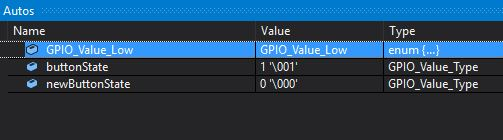
\includegraphics[scale=0.7]{BlinkDebugAuto.JPG}
        \end{figure}
    
    \item Select \textbf{Continue} in the menu bar. Execution pauses again at this breakpoint. Now the value of newButtonState variable is 1, which indicates a button release. Press F9 to remove the breakpoint. Then select \textbf{Continue}. Now, each time press and release Button A, the blink rate changes.
    
    \item To see the messages from the debugger, select \textbf{Debug>Windows>Output} in the dropdown menu.
    
    \item When you are done debugging, select the Stop icon in the menu bar or press Shift+F5.
\end{enumerate}

\subsection{Deploy an application over the air}
This section shows how to create your first over-the-air(OTA) application deplolyment. OTA deployment delivers an application through a feed to the devices in a devices group that match the target stock-keeping unit for the feed.

This section requires:
\begin{itemize}
    \item Your Azure Sphere device is connected to your PC
    \item You have completed all the steps to \autoref{sec:install}
    \item You have completed the previous section and retained the image package for the application
\end{itemize}

\subsubsection{Prepare your device for OTA deployment}
Before you start the OTA deployment process, your Azure Sphere must be ready to accept OTA application updates which means "lock" the device and enable OTA update so that it able to be operated by the customer site. The \textbf{azsphere device prep-field} command is the simplest way to do this. This command:
\begin{itemize}
    \item Disables the ability for Visual Studio to load applications onto the device, so that only OTA applications can be loaded
    \item Assigns a new product SKU to the device
    \item Assigns the device to a new device group that enables OTA application updates
\end{itemize}

The \textbf{azsphere device prep-field} command works on the device that is connected to PC. It has the following form:
\begin{lstlisting}[language=bash]
azsphere device prep-field --newdevicegroupname <unique-dg-name> --newskuname <unique-sku-name>
\end{lstlisting}

The --newdevicegroupname flag specifies a name for the new device group that the command creates. All device groups created by this command support automatic OTA application updates. Supply a descriptive name that is unique among the device group names in your Azure Sphere tenant.

The --newskuname flag specifies a name for the new product SKU that the command creates. A product SKU identifies a model of the connected device that contains an Azure Sphere chip. Each SKU in an Azure Sphere tenant must have a unique name.

The Azure Sphere related to the device has created a device group named "AFSphereGroup" and a product SKU named "AFSphereProductSKU". The command created the group and SKU is:
\begin{lstlisting}[language=bash]
azsphere device prep-field --newdevicegroupname "AFSphereGroup" --newskuname "AFSphereProductSKU"

Removing applications from device.
Component 'e3c4a1ff-8456-49e4-a353-a76235e5136f' deleted or was not present beforehand.
Removing debugging server from device.
Component '8548b129-b16f-4f84-8dbe-d2c847862e78' deleted or was not present beforehand.
Successfully removed applications from device.
Locking device.
Downloading device capability configuration for device ID 'B3E012CE682BA0A6235866AB3A87D838A4817E5C539832A34BF7A715CA8D015FF99C84B909CB2886916259AD186B212E148FC9C4BF8BB6A275A11A2B9495D578'.
Successfully downloaded device capability configuration.
Applying device capability configuration to device.
Successfully applied device capability configuration to device.
The device is rebooting.
Successfully locked device.
Creating a new device group with name 'AFSphereGroup'.
Setting device group ID '5ece1a6b-44b8-40cb-b0e3-623dccd5bc6e' for device with ID 'B3E012CE682BA0A6235866AB3A87D838A4817E5C539832A34BF7A715CA8D015FF99C84B909CB2886916259AD186B212E148FC9C4BF8BB6A275A11A2B9495D578'.
\end{lstlisting}

You aren't required to create a new device group and SKU every time you prepare a device for field use. Typically, you would create one SKU for each product model, and one device group for each collection of devices that you want to update together. To assign the device to different device group use the following command format:
\begin{lstlisting}[language=bash]
azsphere device prep-field --devicegroupid <device-group-id>
\end{lstlisting}
For example, to change the group to AFSphereGroup which created previously, use group id 5ece1a6b-44b8-40cb-b0e3-623dccd5bc6e in the command.

\subsubsection{Link the device to a feed}
The next step is to link your device to a feed that delivers the Blink application. You must supply:
\begin{itemize}
    \item The ID of Azure Sphere OS feed on which the application depends
    \item The path to the image package file that Visual Studio created for the Blink application
    \item A name for the feed that will deliver the application
\end{itemize}

To link to a feed:

\begin{enumerate}
    \item Get the feed ID for the Retail Azure Sphere feed, which delivers the Azure Sphere OS.
    \begin{lstlisting}[language=bash]
    azsphere feed list
    Listing all feeds.
    Retrieved feeds:
    --> [3369f0e1-dedf-49ec-a602-2aa98669fd61] 'Retail Azure Sphere OS'
    --> [82bacf85-990d-4023-91c5-c6694a9fa5b4] 'Retail Evaluation Azure Sphere OS'
    Command completed successfully in 00:00:03.0017019.
    \end{lstlisting}
    Copy the ID of the Retail Azure Sphere OS feed to use in the next step.
    
    \item Issue the azsphere device link-feed command to create a feed and associate it with the Blink image package that you created previously.
    \begin{lstlisting}[language=bash]
    azsphere device link-feed --dependentfeedid 3369f0e1-dedf-49ec-a602-2aa98669fd61 --imagepath "C:\Users\A548068\Documents\AZure\Blink\Mt3620Blink1\Mt3620Blink1\bin\ARM\Debug\Mt3620Blink1.imagepackage" --newfeedname "Mt3620Blink1"
    \end{lstlisting}
    The --dependentfeedid flag supplies the ID of the Retail feed.
    
    The --imagepath flag provides the path to the image package file for the Blink application. The full path to the image file is displayed in the Visual Studio 2017 Build Output windows. The azsphere device link-feed command uploads the image package file to the Azure Sphere Security Service and creates an image set with a unique name.
    
    The --newfeedname flag provides a name for the feed that the command creates. Feed names must be unique in an Azure Sphere tenant, so specify a name that distinguishes this feed from any others.
    
    The outout could be:
    \begin{lstlisting}[language=bash]
    Getting the details for device with ID 'B3E012CE682BA0A6235866AB3A87D838A4817E5C539832A34BF7A715CA8D015FF99C84B909CB2886916259AD186B212E148FC9C4BF8BB6A275A11A2B9495D578'.
    Uploading image from file 'C:\Users\A548068\Documents\AZure\Blink\Mt3620Blink1\Mt3620Blink1\bin\ARM\Debug\Mt3620Blink1.imagepackage':
     --> Image ID:       215c72b6-7472-4337-80c8-da98ef536f39
     --> Component ID:   e3c4a1ff-8456-49e4-a353-a76235e5136f
     --> Component name: 'Mt3620Blink1'
    Removing temporary state for uploaded image.
    Create a new feed with name 'Mt3620Blink1'.
    Adding feed with ID '8354ecb2-5348-4582-9e0c-ae9fc055f3db' to device group with ID '5ece1a6b-44b8-40cb-b0e3-623dccd5bc6e'.
    Creating new image set with name 'ImageSet-Mt3620Blink1-2019.02.22-16.15.07+01:00' for images with these IDs: 215c72b6-7472-4337-80c8-da98ef536f39.
    Adding image set with ID 'e05f2494-a716-48cb-9f41-4d1e1e6fbb7a' to feed with ID '8354ecb2-5348-4582-9e0c-ae9fc055f3db'.
    Successfully linked device 'B3E012CE682BA0A6235866AB3A87D838A4817E5C539832A34BF7A715CA8D015FF99C84B909CB2886916259AD186B212E148FC9C4BF8BB6A275A11A2B9495D578' to feed with ID '8354ecb2-5348-4582-9e0c-ae9fc055f3db'.
    Command completed successfully in 00:00:28.3808069.
    \end{lstlisting}
    
    This command creates a feed that is linked to the device group to which the attached device belongs—that is, the "AFSphereGroup"  created earlier in this quickstart. It will deliver the "Mt3620Blink1" application to all Azure Sphere devices in the group whose product SKU is "AFSphereProductSKU".
\end{enumerate}

\subsection{Update a deployment}
Get the feed ID we created above:
\begin{lstlisting}[language=bash]
    azsphere feed list
    
    Listing all feeds.
    Retrieved feeds:
    --> [3369f0e1-dedf-49ec-a602-2aa98669fd61] 'Retail Azure Sphere OS'
    --> [82bacf85-990d-4023-91c5-c6694a9fa5b4] 'Retail Evaluation Azure Sphere OS'
    --> [8354ecb2-5348-4582-9e0c-ae9fc055f3db] 'Mt3620Blink1'
    Command completed successfully in 00:00:02.2268023.
\end{lstlisting}
Copy the ID of Mt3620Blink1 for the application update.

To update a feed with a new version of your application, use the azsphere component publish command. This command uploads a new image package, creates a new image set, and adds the new image set to an existing feed.

For example, the following command update the Blink Application to the feed just created named Mt3620Blink1:
\begin{lstlisting}[language=bash]
azsphere component publish --feedid 8354ecb2-5348-4582-9e0c-ae9fc055f3db --imagepath "C:\Users\A548068\Documents\AZure\Blink\Mt3620Blink1\Mt3620Blink1\bin\ARM\Debug\Mt3620Blink1.imagepackage" 
\end{lstlisting}

\newpage

\section{Deploy Azure IoT with Azure Sphere}
To use your Azure Sphere devices with the IoT, you can set up an Azure IoT Hub to work with your Azure Sphere tenant. After you have completed the tasks in this section, any device that is claimed by your Azure Sphere tenant will be automatically enrolled in your IoT hub when it first comes online and connects to the Device Provisioning Service (DPS). Therefore, you only need to complete these steps once.

The following sections will guide you to create an IoT Hub with the Azure Sphere.

\subsection{Step 1: Create an Azure IoT Hub and DPS}
\label{subsec:Step1}
This section shows how to set up the Azure cloud resources in the portal for provisioning your devices.

\subsubsection{Create IoT Hub}
This section describes how to create an IoT hub using the \href{https://portal.azure.com}{Azure Portal}
\begin{enumerate}
    \item Log in to the \href{https://portal.azure.com}{Azure Portal}
    \item Choose \textbf{+Create a resource}, then search for \textbf{IoT Hub}.
    \item Click \textbf{Create} button on the left bottom side of the IoT Hub description.
    \begin{figure}[h]
        \centering
        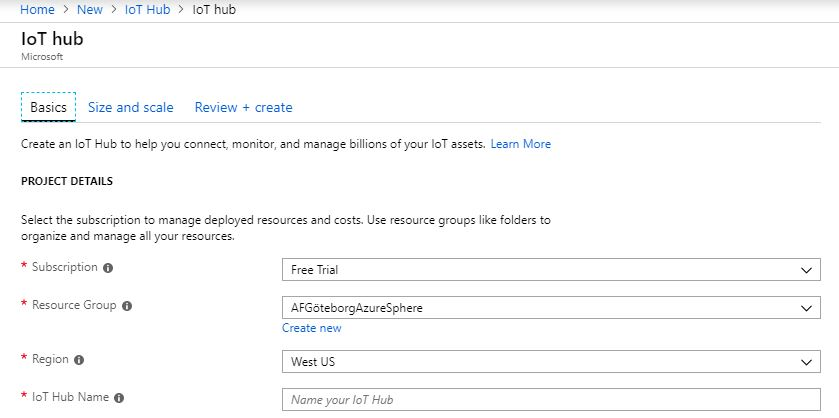
\includegraphics[width=\textwidth]{CreateIoTHub1.JPG}
    \end{figure}
    
    \textbf{Subscription}: Select the subscription to use for your IoT hub.
    
    \textbf{Resource Group}: You can create a new resource group or use an existing one. To create a new one, click Create new and fill in the name you want to use. To use an existing resource group, click Use existing and select the resource group from the dropdown list.
    
    \textbf{Region}: This is the region in which you want your hub to be located. Select the location closest to you from the dropdown list.

    \textbf{IoT Hub Name}: Put in the name for your IoT Hub. This name must be globally unique. If the name you enter is available, a green check mark appears. 
    \newpage
    \item Click \textbf{Next: Size and scale} to continue creating your IoT hub.
    \begin{figure}[h]
        \centering
        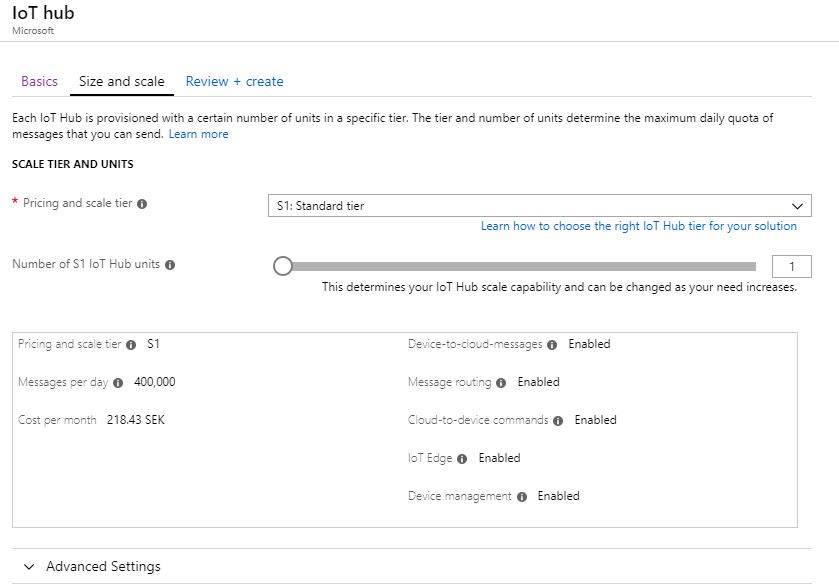
\includegraphics[width=\textwidth]{CreateIoTHub2.JPG}
    \end{figure}
    
    On this screen, you can take the defaults and just click Review + create at the bottom.
    
    \textbf{Pricing and scale tier}: You can choose from several tiers depending on how many features you want and how many messages you send through your solution per day. The free tier is intended for testing and evaluation. It allows 500 devices to be connected to the IoT hub and up to 8,000 messages per day. Each Azure subscription can create one IoT Hub in the free tier.

    \textbf{IoT Hub units}: The number of messages allowed per unit per day depends on your hub's pricing tier. For example, if you want the IoT hub to support ingress of 700,000 messages, you choose two S1 tier units.
    
    \textbf{Advanced / Device-to-cloud partitions}: This property relates the device-to-cloud messages to the number of simultaneous readers of the messages. Most IoT hubs only need four partitions.
    
    \item Click Review + create to review your choices. You should see the similar screen as:
    \begin{figure}[h]
        \centering
        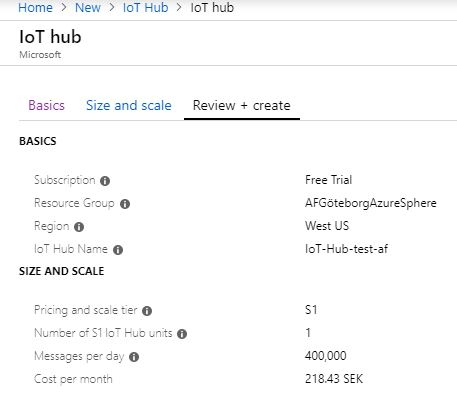
\includegraphics[scale=0.55]{CreateIoTHub3.JPG}
    \end{figure}
    
    \item Click Create to create your new IoT hub. Creating the hub takes a few minutes.
    
    \item In our condition, the IoT Hub has already been created as "azure-temperature-hub", but you can create a new one.
\end{enumerate}


\subsubsection{Create IoT Hub Device Provisioning Service}
\begin{enumerate}
    \item Click the \textbf{Create a resource} button and searching for the \textbf{IoT Hub Device Provisioning Service}. Then click \textbf{Create}
    \item Filling the following information for your new Device Provisioning service and click \textbf{Create}.
          \begin{itemize}
              \item \textbf{Name}: Provide a unique name of the instance. If the name is available, a green check mark appears in the end.
              \item \textbf{Subscription}: Choose the subscription that you want to use to create this Device Provisioning service instance.
              \item \textbf{Resource Group}: You can create a new resource group in this field, or choosing an existing one. 
              \item \textbf{Location}: Select the location to your device.
          \end{itemize}
          \begin{figure}
            \centering
            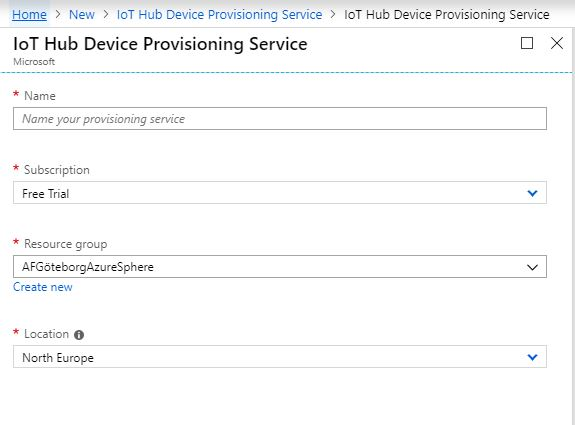
\includegraphics[scale=0.45]{DeviceProvisioningService.JPG}
          \end{figure}
    \item Once the service is successfully deployed, the notifications will notify you, then click \textbf{Go to resource}
    \item In our condition, the name of the provision is "afgoteborg-azure-provision"
\end{enumerate}

\subsubsection{Link the IoT Hub and Device Provisioning Service}
This section describes the configuration in the Device Provisioning Service sets the IoT hub for the devices will be provisioned.
\begin{enumerate}
    \item Click the \textbf{All resources} button from the left-hand menu of the Azure portal. Select the Device Provisioning service that you created in the preceding section.
    \item Under the settings, select Linked IoT hubs. Then click \textbf{+Add}. 
    \item In the \textbf{Add link to IoT hub}, provide the following information to link your new Device Provisioning service instance to an IoT hub. Then click Save.
          \begin{itemize}
              \item \textbf{Subscription}: Select the subscription containing the IoT hub that you want to link with your new Device Provisioning service instance.
              \item \textbf{Iot hub}: Select the IoT hub to link with your new Device Provisioning service instance.
              \item \textbf{Access Policy}: Select iothubowner as the credentials for establishing the link with the IoT hub.
          \end{itemize}
          \begin{figure}
            \centering
            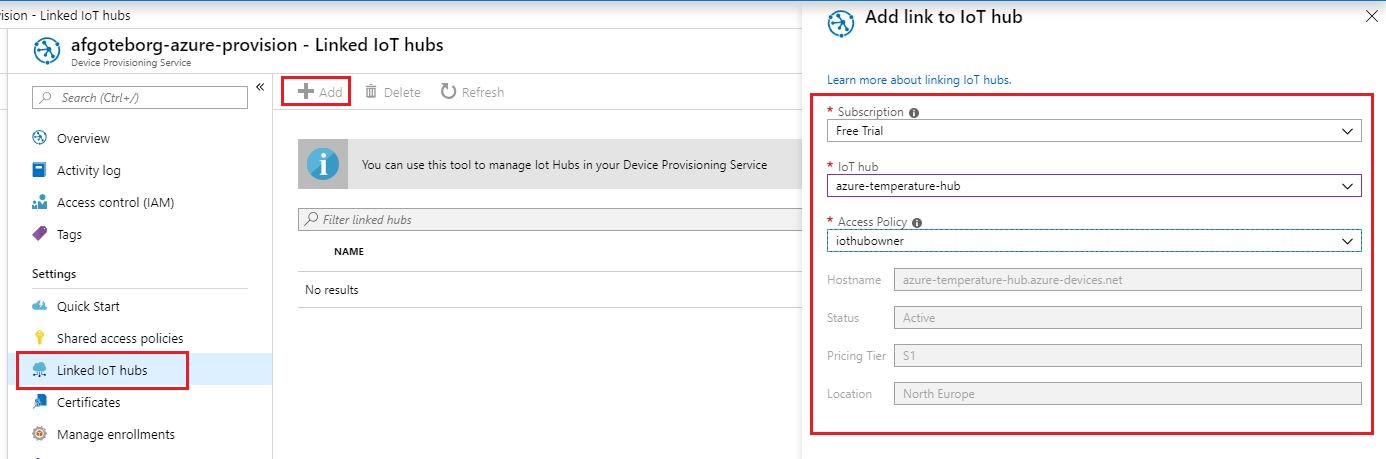
\includegraphics[width=\textwidth]{LinkIoT.JPG}
      \end{figure}
      \item You should be able to see the newly created Linked IoT hubs in the list.
\end{enumerate}

\subsubsection{Clean up resources}
If you want to continue on this tutorial, you do not need to do this step. If you are not, use the following steps to delete the resources just created.
\begin{enumerate}
    \item From the left-hand menu in the Azure portal, click \textbf{All resources} and then select your Device Provisioning service. At the top of the \textbf{All resources} blade, click \textbf{Delete}.
    \item From the left-hand menu in the Azure portal, click \textbf{All resources} and then select your IoT hub. At the top of the All resources blade, click \textbf{Delete}.
\end{enumerate}

\subsection{Step2: Download the tenant authentication}
After finished the previous section, we can set up the Azure Sphere device with the IoT.
\begin{enumerate}
    \item Open the Azure Sphere Developer Command Prompt in the Start menu.
    \item Sign in with the user for your Azure Active Directory:
    \begin{lstlisting}[language=bash]
        azsphere login
    \end{lstlisting}
    \item Download the Certificate Authority (CA) certificate for your Azure Sphere tenant, the output file must have the .cer extension.
    \begin{lstlisting}[language=bash]
        azsphere tenant download-CA-certificate --output AFTechCert.cer
    \end{lstlisting}
\end{enumerate}

\subsection{Step3: Upload the tenant CA certificate to DPS and generate a verification code}
\begin{enumerate}
    \item Log in to the \href{https://portal.azure.com}{Azure Portal} and navigate to the  DPS(Device Provisioning Service) you created in \ref{subsec:Step1}
    \item Open \textbf{Certificates} from the menu. 
    \begin{figure}[h]
        \centering
        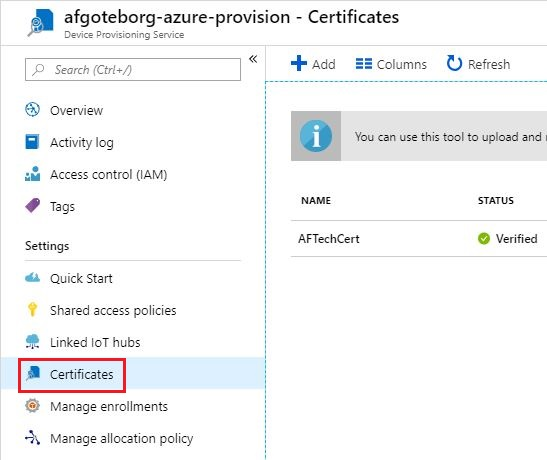
\includegraphics[scale=0.6]{DPSCert.JPG}
    \end{figure}
    \newpage
    \item Then click \textbf{ADD} to add a new certificate and enter a name for your certificate. Upload the .cer file from Step 2.
    \begin{figure}[h]
        \centering
        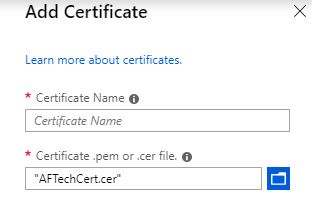
\includegraphics[scale=0.7]{DPSAddCert.JPG}
    \end{figure}
    \item After you are notified that the certificate uploaded successfully, click \textbf{Save}.
    \item The new certificate is listed under the explorer. Note the STATUS of the certificate is Unverified. Click on this certificate.
    \begin{figure}[h]
        \centering
        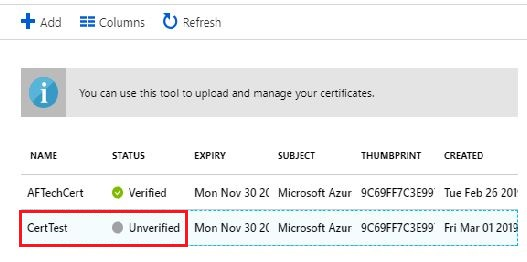
\includegraphics[scale=0.7]{DSPCertUnVer.JPG}
    \end{figure}
    \item In \textbf{Certificate Details}, click Generate Verification Code. The DPS creates a Verification Code that you can use to validate the certificate ownership. Copy the code to your clipboard for use in the next step.
    
\end{enumerate}

\subsection{Step 4: Verify the tenant CA certificate}
\begin{enumerate}
    \item Back to the Azure Sphere Developer Command Prompt. Download the validation certificate based on your own tenant CA certificate. Replace code in the command with the verification code from the previous setp.
    \begin{lstlisting}[language=bash]
        azsphere tenant download-validation-certificate --output AFTechValidationCert.cer --verificationcode <code>
    \end{lstlisting}
    The Azure Sphere Security Service signs the validation certificate with the verification code from the DPS to your own CA.
    \item Return to the Azure Portal to upload the validation certificate to DPS. In \textbf{Certificate Details}, use the File Explorer icon next to the \textbf{Verification Certificate .pem or .cer file} field to upload the signed verification certificate. Then click \textbf{Verify}.
     \begin{minipage}{.45\textwidth}
        \centering
        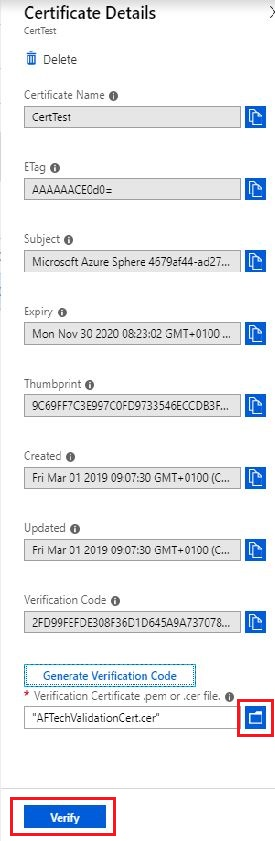
\includegraphics[scale=0.8]{CertificatDetails.JPG}
    \end{minipage}
    \item The \textbf{STATUS} of the certificate changes to \textbf{Verified} in the list. Click \textbf{Refresh} if it does not update automatically.
\end{enumerate}
\newpage
\subsection{Step 5: Use the certification to add you device to and enrollment group}
\begin{enumerate}
    \item In the same DPS view as previous step. Select \textbf{Manage enrollment}, then click \textbf{Add enrollment group}.
    \item In the Add Enrollment Group panel, create a name for your enrollment group, select CA Certificate as the \textbf{Certificate type}, and select the certificate that you validated in the previous step.
    \item Click \textbf{Save}. You should see the group name appears under the \textbf{Enrollment Group} on the successful creation of the enrollment group.
    \begin{figure}[h]
        \centering
        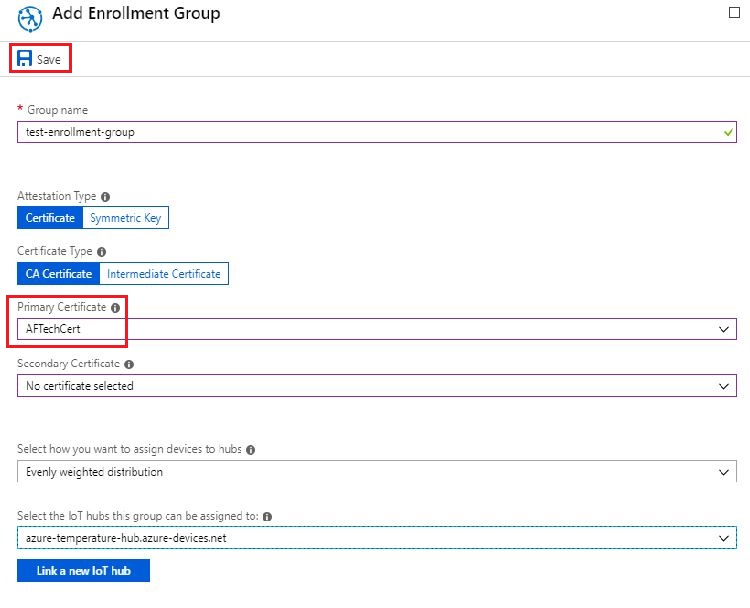
\includegraphics[scale=0.5]{EnrollmentGroup.JPG}
    \end{figure}
\end{enumerate}

\subsection{Azure Sphere IoT Hub Sample Application}
The Azure IoT Hub sample application shows the communication between the Azure IoT Hub and the Azure Sphere Device.

This sample uses the Connected Service for Azure Sphere, which is installed with the Azure Sphere SDK. The Visual Studio provides a template for connecting
the Azure Sphere device to your IoT hub and communication with the hub. Application that use the Connected Service functionality can send messages to and 
receive messages from and IoT Hub, maintain a device twin, and direct method calls from cloud service.

This sample does the following:
\begin{enumerate}
    \item Displays the currently connected WiFi network
    \item Blinks LED 1 constantly. Pressing button A changes the rate. The rate is also stored in the device twin so that a cloud service program can change it.
    \item Sends a message to the IoT Hub when you press button B.
    \item Lights LED 3 green after start-up to indicate that the device has connected to the IoT Hub and the application has successfully authenticated with the hub.
    \item Changes the color of LED 1 in response to a direct method call.
\end{enumerate}

You must set up the board:
\begin{enumerate}
    \item Connect to a PC and to WiFi network.
    \item Change the board to prep-debug.
\end{enumerate}

\subsubsection{Add the device to the IoT hub}
\begin{enumerate}
    \item Start Visual Studio 2017 and go to \textbf{File>New>Project}. Navigate to the template in \textbf{Visual C++>Cross Platform>Azure Sphere}. Select Azure IoT Hub Sample for MT3620 RDB (Azure Sphere), specify a name and location or use the defaults, and select OK.
    \item In Solution Explorer, right click on \textbf{Reference} and then select \textbf{Add Connected Service}
    \begin{figure}[h]
        \centering
        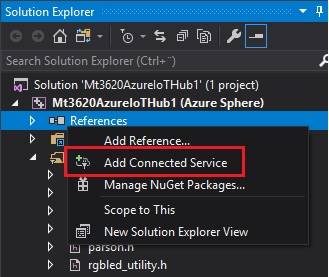
\includegraphics[scale=0.6]{VSAddConnectService.jpg}
    \end{figure}
    \item Select \textbf{Device Connectivity with Azure IoT} from the list of connected services.
    \begin{figure}[h]
        \centering
        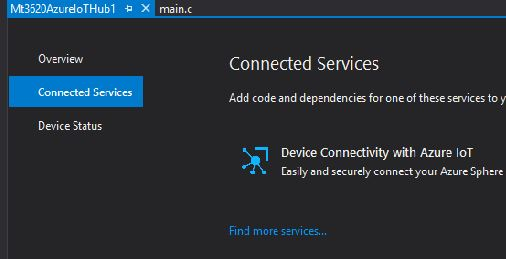
\includegraphics[scale=0.5]{AddConServiecPan.JPG}
    \end{figure}
    \item It may ask you to log in to the account you're using with your Azure Sphere tenant.
    \item In the Device Connectivity, select your Azure subscription from the \textbf{Subscription} dropdown. Select Device Provisioning Service from the \textbf{Connection Type} dropdown. Select your Device Provisioning Service from the \textbf{Device Provisioning Service} dropdown.
    \begin{figure}[h]
        \centering
        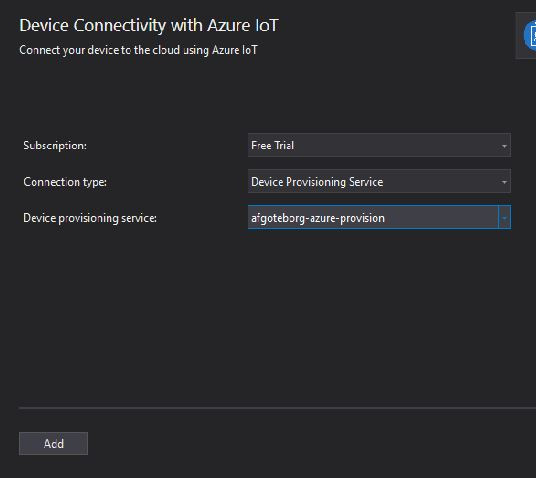
\includegraphics[scale=0.5]{CreateDiveConIoT.JPG}
    \end{figure}
    \item Click Add.
    \item In Solution Explorer, you should now see azure\_iot\_utilities.h and azure\_iot\_utilities.c in your solution. In addition, the host name for the Azure IoT Hub has been added to the Capabilities section of the app\_manifest.json file. An application can connect only to the internet hosts that are specified in the AllowedConnections field.
    \begin{figure}[h]
        \centering
        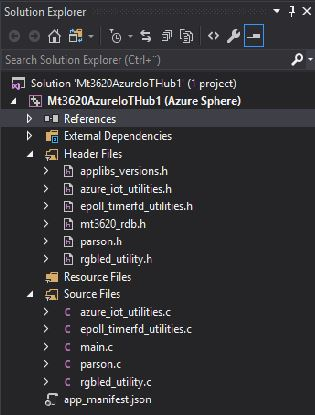
\includegraphics[scale=0.55]{IoTSolutionExplorer.JPG}
    \end{figure}
\end{enumerate}

\subsubsection{Start the Sample}
\begin{enumerate}
    \item Open main.c in the sample application
    \item Press F5 to build, load and start the sample.
    
    The sample opens the handles to the buttons and the RGB LEDs, it also displays the connected WiFi network.

    Then it starts the main loop. You should see LED 1 start to blink and see output like the following in the Output window:
    \begin{figure}[h]
        \centering
        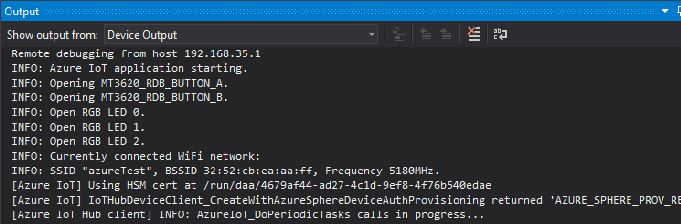
\includegraphics[scale=0.7]{ASIoTOutput.JPG}
    \end{figure}
\end{enumerate} 

\subsubsection{Send and receive messages}
In Azure Portal you can send and receive the messages from your device.
\begin{enumerate}
    \item Log in to Azure Portal with the IoT Hub we created previously.
    \item Select \textbf{All Resources} on the left panel. Click on the IoT hub in the resource list.
    \item Navigate to \textbf{IoT devices} in the Explorers section in the IoT Hub panel. You may need to scroll down a little bit.
    \begin{figure}[h]
        \centering
        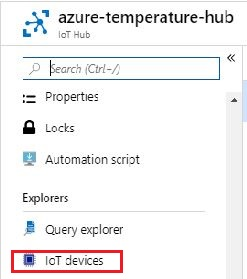
\includegraphics[scale=0.65]{SelectIoTDevice.JPG}
    \end{figure}
    \item You should see the device id in the list. Click on the device id to open the \textbf{Device details} panel.
    \item Click on the \textbf{Message to device}. In the \textbf{Message to device} type some messages, for example "Hello from Portal" in the \textbf{Message Body} textbox. Then click \textbf{Send Message}.
    \begin{figure}[h]
        \centering
        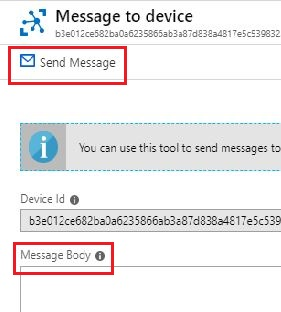
\includegraphics[scale=0.6]{MsgToDevice.JPG}
    \end{figure}
    Back to Visual Studio 2017, in the output Windows you should see a message \textbf{[Azure IoT] INFO: Received message 'Hello from Portal' from IoT Hub} coming out in the output windows.
\end{enumerate}

\subsubsection{Call a direct method on the device}
\begin{enumerate}
    \item Back to Device Details in the portal. You may see the prompt said "Your unsaved edit will be discarded", click \textbf{OK}. Then select \textbf{Direct method}.
    \item In the \textbf{Direct method} panel, fill in \textbf{LedColorControlMethod} under the \textbf{Method Name} box, and \textbf{{"color":"green"}} in the Method payload box. Then click \textbf{Invode Method}.
    \begin{figure}[h]
        \centering
        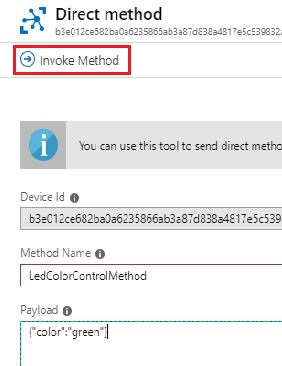
\includegraphics[scale=0.7]{DirectMethod.JPG}
    \end{figure}
    \item You should see the following output in the Visual Studio output window and LED 1 start blinking green.
    \begin{lstlisting}[language=bash]
    [Azure IoT] INFO: Trying to invoke method LedColorControlMethod
    INFO: LED color set to: 'green'.
    \end{lstlisting}
    In the meantime, check the Result in the Direct Method in the portal, the return payload should be 
    \begin{lstlisting}[language=bash]
    {"success":true,"message":"led color set to green"}
    \end{lstlisting}
\end{enumerate}

\subsubsection{Manage a device twin}
A device twin is a JSON document in the cloud that stores information about a device. Use the device twin to synchronize status information and maintain device properties that should be accessible to cloud service applications as well as to applications that run on the device.
\begin{enumerate}
    \item Back to Device Details in the portal. Then select \textbf{Device twin}.
    \item You should see the JSON document in the panel. Find \textbf{LedBlinkRateProperty} under \textbf{desired} properties, if you cannot find it, please add it before \textbf{metadata}. Set the value 0, 1 or 2.
    \item Then click \textbf{Save}.
    \begin{figure}[h]
        \centering
        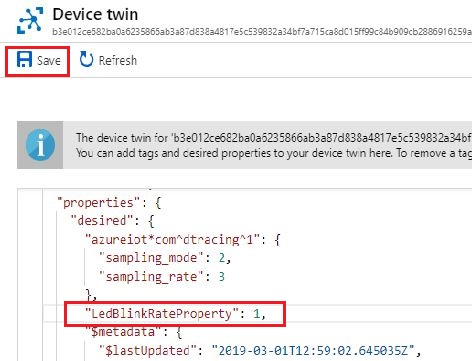
\includegraphics[scale=0.7]{DeviceTwin.JPG}
    \end{figure}
    \item In Visual Studio, check the Output window. You should see:
    \begin{lstlisting}[language=bash]
    INFO: Received desired value 1 for LedBlinkRateProperty, setting it to 1.
    [Azure IoT] INFO: Set reported property 'LedBlinkRateProperty' to value 1.
    \end{lstlisting}
    In the meantime, the blinking rate of the LED 1 should be changed.
\end{enumerate}
\newpage

\section{Azure Sphere Read AM2302}
This section will explain the functions to read the sensors data from a AM2302. Due to the specific GPIO function in Azure Sphere, it may not able to read the one-wire sensor, such as the AM2302. To have a work around, the sensor connects to an Arduino device, and send the sensor data through UART to Azure Sphere. 

This section assume you already have:
\begin{itemize}
    \item Your Azure Sphere device is connected to your PC
    \item You have completed all the steps to \autoref{sec:sim_app}
    \item You have git command installed in a PC.
    \item You have Visual Studio 2017
    \item You have Arduino IDE
\end{itemize}

\subsection{Connect Azure Sphere to Arduino and AM2302}
The Azure Sphere communicates with Arduino through UART. The UART pins on Azure Sphere are PIN1(RXD0) and PIN3(TXD0) in Header 2. The wirings are:  
\begin{itemize}
    \item Arduino TX(PIN1)->AzureSphere RXD0(Header2, PIN1)
    \item Arduino RX(PIN0)->AzureSphere TXD0(Header2, PIN3)
\end{itemize}

The diagram shows how to connect them. 
\begin{figure}[h]
    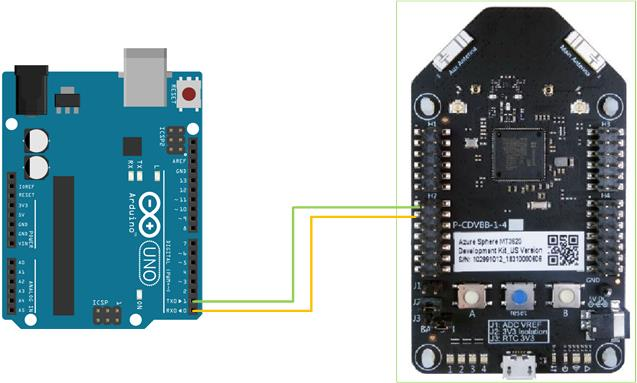
\includegraphics[scale=0.7]{AStoAD.jpg}
\end{figure}

Connecting Arduino to the AM2302 is fairly straight forward, there are three cables to AM2303, red cable to VCC(3.3v/5v), black cable to GND and yellow cable is the signal out, in this project it connects to PIN2.
The diagram shows how to connect the Arduino with AM2302:
\begin{figure}[h]
    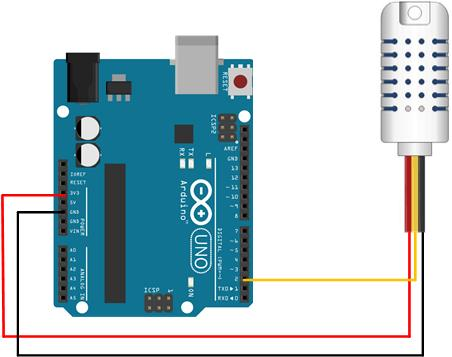
\includegraphics[scale=0.6]{ADtoAM2302.jpg}
\end{figure}

\subsection{Clone the code from Github}
The code can be download from Github using following command:
\begin{lstlisting}[language=bash]
git clone https://github.com/jianyuanMa/AzureSphereDHT22.git
\end{lstlisting}

\subsection{Some Explanations about the project}
The project has two parts. First part is the Arduino read the sensor data periodically and send it to the UART while the Azure Sphere receives the data as the second part.

\subsubsection{Read Sensor Data in Arduino}
Open Arduino IDE in the Start menu and open the file UartAM2302.ino in the folder ArduinoCode. The sensor reading uses the library from Adafuit. To install the library, select \textbf{Sketch>Include Library>Manage Libraries} in the dropdown menu. 

Enter "DHT" in the search field and look through the list for “DHT sensor library by Adafruit.” Click the “Install” button, or “Update” from an earlier version.
\begin{figure}[h]
    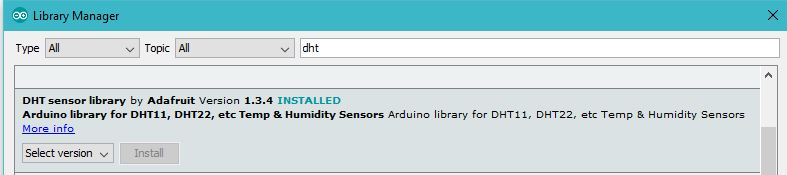
\includegraphics[scale=0.6]{DHTLibary.JPG}
\end{figure}

You also need to install the Adafruit\_Sensor library, which is also available in the Arduino Library Manager.
\begin{figure}[h]
    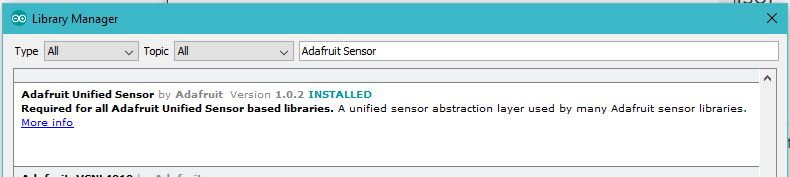
\includegraphics[scale=0.6]{AdafruitUnifiedSensor.JPG}
\end{figure}

\subsubsection{Communicate through UART}
The second part is communication between the Arduino and Azure Sphere through UART. Open Visual Studio 2017 and select \textbf{File->Open->Project/Solution}. In the open dialogue, navigate to the Git repository we just downloaded and select the file "AzureArdruino.sln" to open the Visual Studio Project.

This project is referenced to the \textbf{UART Sample for MT3620 RDB(Azure Sphere)}, you find it by select \textbf{Fild>New Poject>Visual C++>Cross Platform>Azure Sphere}.

To use the UART read function, it needs to include the "applibs/uarts.h" library. The funtion "UartEventHandler" reads the messages whenever they have been sent from the Arduino. Since we know the messages are the sensor data from AM2302 in an array format {humidity,temperature}. We can easily convert each message into the actual numbers and ready for uploading to the cloud. The function "charArrayToNumbers" helps to achieve that.

\subsection{Test the Output}
\begin{enumerate}
    \item Connect Arduino to a PC and start the Arduino IDE. Then open the UartAM2302.ino.
    
    \item Select \textbf{Tools>Port} then looking for the port with the description \textbf{Arduino/Genuino Due}.
    
    \item Click Upload \inlinegraphics{UploadBTArduino.JPG} in the tool bar. If you see the output similar to the following, it means the program has been successfully uploaded to the Arduino.
    \begin{lstlisting}[language=bash]
Sketch uses 5682 bytes (17%) of program storage space. Maximum is 32256 bytes.
Global variables use 191 bytes (9%) of dynamic memory, leaving 1857 bytes for local variables. Maximum is 2048 bytes.
    \end{lstlisting}
    
    \item Connect the Azure Sphere to a PC. Prepare the board to enable the debug from a PC.
    \begin{lstlisting}[language=bash]
    azsphere device prep-debug
    \end{lstlisting}
    
    \item Open the \textbf{AzureArduino.sln} in Visual Studio 2017. Then select the \textbf{Remote GDB Debugger} in the tools bar to start the debug process.
    
    \item You should be to see the output in the Output window like:
    \begin{lstlisting}[language=bash]
Remote debugging from host 192.168.35.1
UART application starting.
Opening MT3620_RDB_LED2_RED.
Humidiy 18.70, Temperature 22.10
Humidiy 18.70, Temperature 22.10
......
    \end{lstlisting}
    
\end{enumerate}

\section{Future Work}
This tutorial is just a startup guide about the Azure Sphere device, Azure Security Services and the IOT. To have a complete demo 
about the Azure Sphere, there are still a lot of work to be done and some questions need to be solved.

\subsection{Remain Questions}
\begin{enumerate}
    \item The device was claimed under Jianyuan Ma's ÅF account, in the ÅF directory, because there is a tenant named "AFTechnology". 
          Please reference to the \ref{sec:install}. We have figure out how to create the tenant under directory "af sphere" and claim 
          a new device.
    \item The temperature reading is not read by the Azure Sphere device but the Arduino, due to the GPIO pins on Azure Sphere can not 
          change the mode after they have been opened and occupied. Jianyuan Ma did not find the best solution to operate the AM2302 
          sensor by Azure Sphere. 
\end{enumerate}

\subsection{Remain Works}
\begin{enumerate}
    \item Create an IoT service for the sensor reading from Azure Sphere.
    \item Setup a message routing in the IoT hub to receive the messages from Azure Sphere. The message routing can be found under the 
          IoT hub created in the \ref{subsec:Step1}. You may need to scroll down a little bit. The tutorial on how to create the messages
          routing can be found in \href{https://docs.microsoft.com/en-us/azure/iot-hub/tutorial-routing}{Configure message routing with IoT Hub}, 
          you may need to create a Service Bus Queue also, which can be found in \href{https://docs.microsoft.com/en-us/azure/service-bus-messaging/service-bus-dotnet-get-started-with-queues}{Get started with Service Bus queues}
    \item Create a web application to display the sensor messages into a diagram.
    \item Further studies on Azure Sphere, such as the \href{https://docs.microsoft.com/en-us/azure-sphere/deployment/deployment-overview}{Over-the-Air Deployment} and 
          other resources in the Azure Portal.
    \item The \href{http://wiki.seeedstudio.com/Azure_Sphere_MT3620_Development_Kit/}{Azure Sphere MT3620 Development Kit} might be a 
          very helpful to understand the Azure Sphere device, IoT hub, OTA application and Security Services.
\end{enumerate}
\newpage

\end{document}
